\section{PoE SNMP Monitoring Tool}
\label{sec:tool}
Diese Sektion beschreibt das durch das Projektteam entwickelte Tool welches für das PoE Monitoring verwendet wird.
Hierfür wird neben der Beschreibung der Oberfläche auch Details über den Aufbau des Tools illustriert.

\subsection{Architektur}

Das PoE-Tool besteht grundsätzlich aus drei Komponenten (beziehungsweise vier wenn man die Datenbank mit zählt), welche in Abbildung \ref{fig:architecture} dargestellt werden. 

\begin{figure}[h]
    \centering
    \leavevmode
    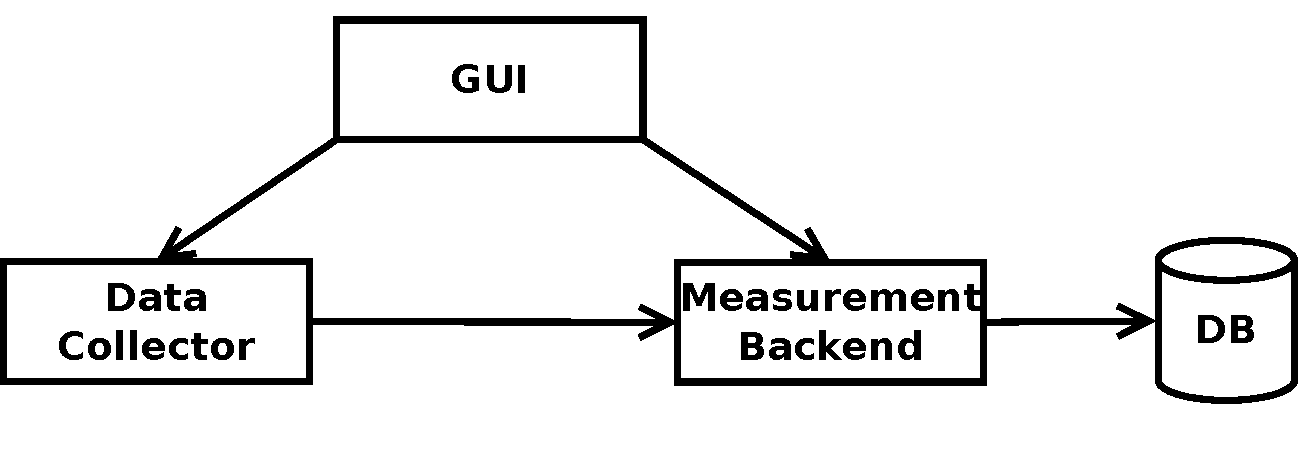
\includegraphics[width=1.0\linewidth]{figures/architecture_new}
    \caption{Software-Architektur PoE SNMP Monitoring Tool}
    \label{fig:architecture}
\end{figure}

Die Funktionen der einzelnen Komponenten ist wie folgt eingeteilt:

\begin{description}
  \item[Measurement Backend:] Diese Komponente bildet die Schnittstelle des Systems zu der Datenbank welche für die Speicherung der Nutzdaten des Tools verwendet wird. Diese Komponente bietet Funktionen zum Anlegen, Speichern und Löschen von Switches, Speichern von Messungen und dem Abfragen dieser durch verschiedenste Kriterien.
  \item[Data Collector:] Diese Komponente ist für die kontinuierliche Abfrage (die Intervalle werden im Config-File angegeben) von Messungen für alle aktiven Switches verantwortlich. Während jeder Messung wird der aktuelle PoE Status jedes Ports pro Switch ausgelesen. Nachdem die Werte aller Ports eines Switches ausgelesen wurden, werden die entsprechenden Messungen an das \textbf{Measurement Backend} zum Speichern eben dieser gesendet.
  \item [GUI] Die GUI-Komponente nimmt Benutzeranfragen entgegen und fragt die darzustellenden Daten vom \textbf{Measurement Backend} ab. Das \textbf{Measurement Backend} liefert die entsprechenden Daten die dann in ein übersichtliches, von Menschen verwertbares, Datenmaterial konvertiert und angezeigt werden.
\end{description}

\subsection{Konfiguration}

Das PoE-Tool wird über die Konfigurationsdatei \textbf{config.properties} angepasst. Diese enthält folgende Optionen:

\begin{description}
  \item [measurement.interval] Dieser Wert gibt die Zeit in Millisekunden an, die zwischen zwei Messungen des selben Switches vergehen sollen. Dieser Wert muss je nach Struktur des Netzwerks gewählt werden, da hier auch die Zeit die der Switch zum Antworten auf SNMP Anfragen braucht eingerechnet werden muss. Ein zu kleiner Wert raubt den Messungen die Aussagekraft.
  \item [distribution.slots] Basierend auf diesem Wert, wird das Zeitintervall, welches in \textbf{measurement.interval} definiert ist, in x Zeitslots eingeteilt. Diese Einstellung wurde eingeführt, damit nicht alle Switches immer zur gleichen Zeit befragt werden und statt dessen eine bessere Verteilung der Anfragen gewährleistet wird. Zum Beispiel: Intervall ist auf 1000 ms und Slots auf 10 eingestellt. Daraufhin wird das Intervall in 10 Slots aufgeteilt, die 100 ms von einander entfernt sind.
  \item [\textbf{data.retriever.impl}] Dieser Wert gibt an welche Implementierung des SNMP\-Data\-Retriever-Interfaces zu verwenden ist, welche verwendet wird um eine Messung via SNMP durchzuführen. Derzeit gibt es zwei Implementierungen dieses Interfaces:
  \begin{description}
   \item[cn.poe.group1.collector.DummyDataRetriever:] Ist eine Testimplementierung welche das Laden von SNMP Werten nur simuliert und Testwerte zurück gibt. Wurde für die Erstellung des Prototyps verwendet.
   \item[cn.poe.group1.collector.DataRetriever:] Ist die reale Implementierung welcher wirklich SNMP Werte von Geräten abfragt.
  \end{description}
\end{description}

\subsection{Verwendung}
Beim Start des PoE-Tool wird die Datenbank auf existierende Switch Definitionen überprüft. Für jede existierende Definition, wird automatisch mit den Messungen für den entsprechenden Switch begonnen. Danach wird das GUI des Tools gestartet, welche alle existierenden Definitionen in der linken Tabelle anzeigt. Wird ein Switch dort ausgewählt, werden seine Nutzdaten im rechten Feld angezeigt.

Wichtig: Die GUI zeigt immer nur die Messdaten aus einem bestimmten Zeitraum an. Dieser kann im Hauptfenster rechts oben definiert werden. Um die Nutzdaten zu aktualisieren, muss der \textbf{Reload} Button betätigt werden.

\subsubsection{Switch}
Durch die Auswahl eines Switches in der linken Tabelle, werden die entsprechenden Nutzdaten geladen. Hierbei sind die Nutzdaten kategorisch auf zwei Registerkarten aufgeteilt:
\begin{description}
 \item[Ports:] Die Werte in dieser Registerkarte listen die Durchschnittszahlen für die PoE Werte der Ports des gewählten Switches auf. Auf diese Weise kann ein schneller Überblick über alle Ports gewährleistet werden. Dieser Reiter wird immer beim Öffnen eines Switches als Standard angezeigt. Details über die Ports werden in Punkt \ref{sub:ports} genauer erläutert.
 \item[Switch:] Dieser Reiter bietet eine Übersicht über die kumulierten Werte der Ports des gewählten Switches in Form einer Kurve. Somit bietet diese Sicht einen guten Überblick über den PoE Werteverlauf des gesamten Switches und erlaubt eine schnelle Überprüfung der Kapazitätsgrenzen des Switches (siehe Abbildung \ref{fig:overview-switch}).
\end{description}

\begin{figure}[h]
    \centering
    \leavevmode
    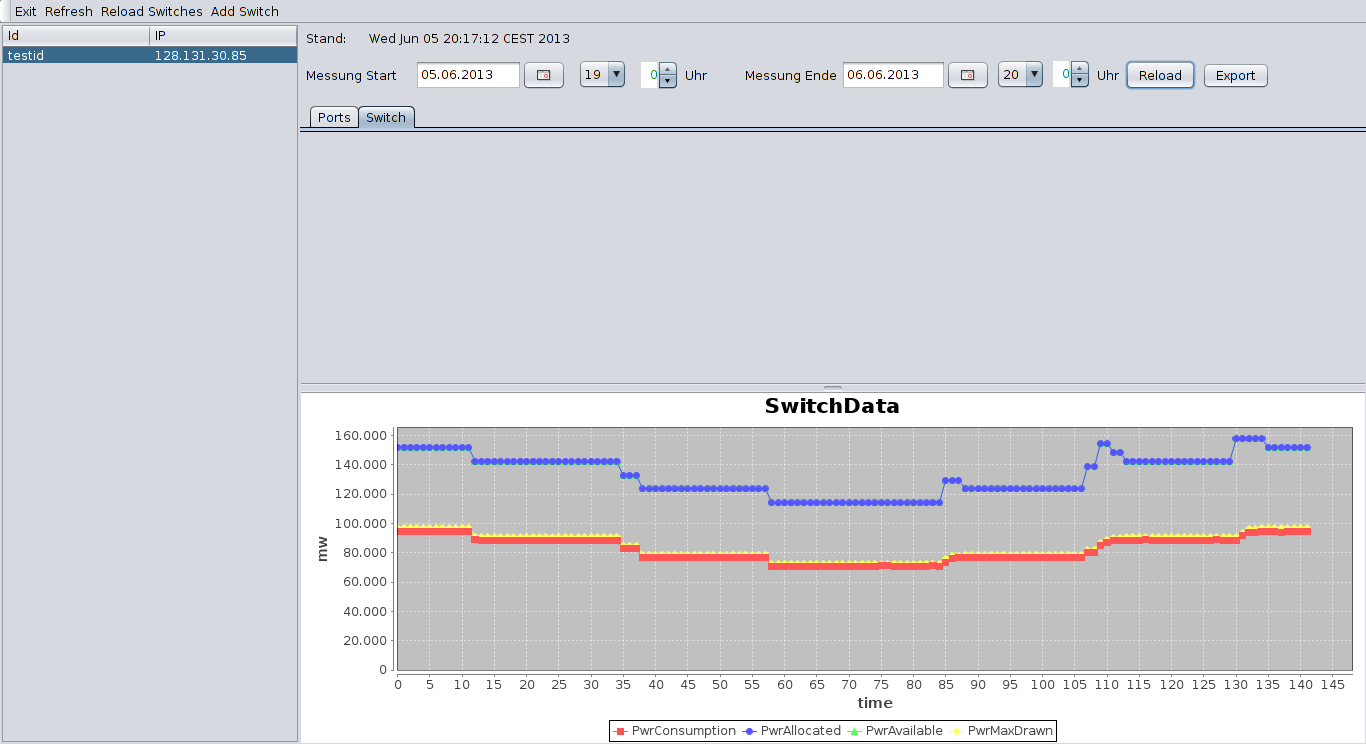
\includegraphics[width=1.0\linewidth]{figures/switchDetails}
    \caption{Übersicht über einen Switch}
    \label{fig:overview-switch}
\end{figure}

Um einen neuen Switch, welcher überwacht werden soll, zu dem Tool hinzuzufügen, gibt es den Menüpunkt \textbf{Add Switch} in der Menüleiste des Tools. Durch aktivieren dieses Menüpunktes, wird ein Popup geöffnet (siehe Abbildung \ref{fig:popup}) welches ausgefüllt und bestätigt werden muss. Nach dem Anlegen eines neuen Switches, beginnen die Messungen automatisch im Hintergrund.

 \begin{figure}[h]
    \centering
    \leavevmode
    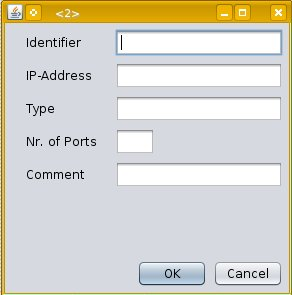
\includegraphics[scale=0.5]{figures/screenshot3}
    \caption{Popup um neuen Switch anzulegen}
    \label{fig:popup}
\end{figure}

Um Switches editieren beziehungsweise löschen zu können, wurden diese Funktionen in das Kontextmenü der linken Tabelle hinzugefügt. Das Kontextmenü enthält einen Punkt zur Änderung des Switches (\textbf{Edit Switch}) und ein Punkt für das Löschen von Switches (\textbf{Delete Switch}).

\subsubsection{Ports}
\label{sub:ports}
Auf der Registerkarte Ports im rechten Teil des Fensters können die Daten über die einzelnen Ports eines Switches betrachtet werden. Die Tabelle enthält dabei einen Mittelwert aus den Messungen über die einzelnen Parameter für den gegebenen Zeitraum. Das Diagramm enthält einen graphischen Verlauf der einzelnen Parametern. Abbildung \ref{fig:overview-port} zeigt wie die Port Übersicht im Tool aussieht.

\begin{figure}[h]
    \centering
    \leavevmode
    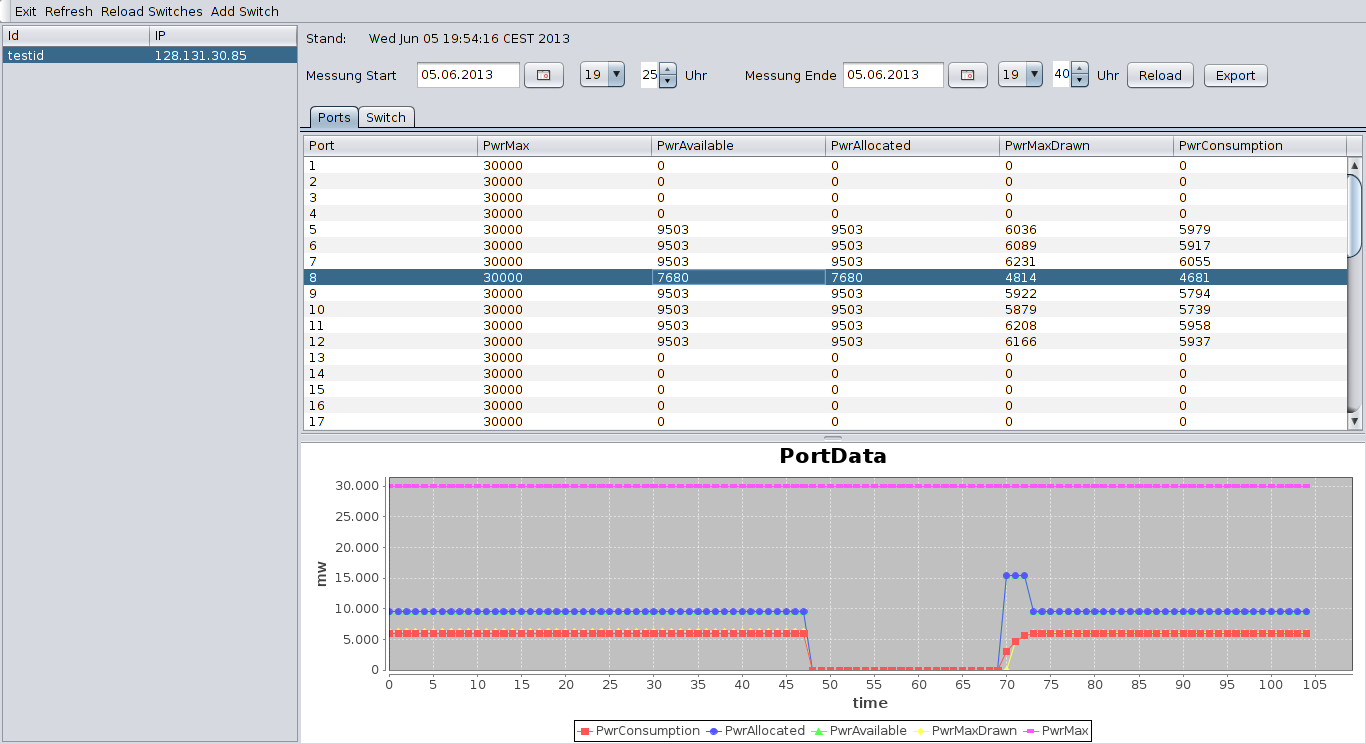
\includegraphics[width=1.0\linewidth]{figures/portDetails}
    \caption{Übersicht über einen Port}
    \label{fig:overview-port}
\end{figure}

\subsubsection{CSV Export}
Durch einen Klick auf den Button \textbf{Export} können sämtliche Messungen, welche im angegebenen Zeitraum für den ausgewählten Switch gemacht wurden, in eine CSV-Datei exportiert werden. Durch betätigen des \textbf{Export} Buttons, wird ein Datei-Dialog angezeigt, in welchen man Ort und Name der resultierenden CSV-Datei angeben muss.
